\documentclass[titlepage]{article}

\usepackage[letterpaper,margin=1in,footskip=0.25in]{geometry}
\usepackage[hidelinks]{hyperref}
\usepackage{fancyhdr}
\usepackage{csquotes}
\usepackage{tikz}
\usepackage[list=true]{subcaption}
\usepackage{graphicx}

\MakeOuterQuote{"}

\usetikzlibrary{knots}

\newcommand{\dq}[2]{``#1" (#2).}

\title{{\Huge\emph{The Knot Book}}\\[5pt]\textcolor{gray!60!black}{Notes}\vspace{-0.5em}}
\author{Steven Labalme}
\date{\today}

\begin{document}




\pagenumbering{gobble}
\maketitle



\pagenumbering{roman}
\tableofcontents
\listoffigures
\listoftables
\newpage



\pagenumbering{arabic}
\pagestyle{fancy}
\fancyhf{}
\rfoot{Labalme \thepage}
\renewcommand{\headrulewidth}{0pt}
\section{Introduction}\label{sse:intro}
\subsection{Introduction}
\begin{itemize}
    \item \textbf{Knot}: \dq{A knotted loop of string, except that we think of the string as having no thickness, its cross-section being a single point}{2}
    \item Do not distinguish between a `nice, even' knot and one that has been deformed through space.
    \item \textbf{Unknot}: \dq{The simplest knot of all\dots the unknoted circle}{2} \emph{Also known as} \textbf{trivial knot}. See Figure \ref{fig:circletrefoila}.
    \item \textbf{Trefoil knot}: \dq{The next simplest knot}{2} See Figure \ref{fig:circletrefoilb}.
    \begin{figure}[h!]
        \centering
        \begin{subfigure}{0.2\linewidth}
            \centering
            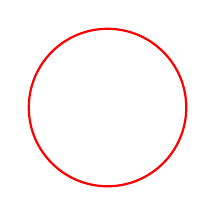
\begin{tikzpicture}
                \draw[red,thick] (0,0) circle (1cm);
            \end{tikzpicture}
            \caption{Trivial knot.}
            \label{fig:circletrefoila}
        \end{subfigure}
        \begin{subfigure}{0.2\linewidth}
            \centering
            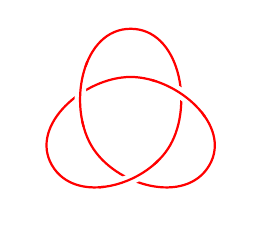
\begin{tikzpicture}
                \begin{knot}[
                    consider self intersections,
                    clip width=5
                ]
                    % could be defined with a combination of polar coordinates and foreach...
                    \strand[red,thick] (1,{3^0.5})
                        to [out=0,in=60] (1.5,0.25)
                        to [out=240,in=-60] (0,0)
                        to [out=120,in=180] (1,1.12)
                        to [out=0,in=60] (2,0)
                        to [out=240,in=-60] (0.5,0.25)
                        to [out=120,in=180] cycle
                    ;
                    \flipcrossings{1,3}
                \end{knot}
            \end{tikzpicture}
            \caption{Trefoil knot.}
            \label{fig:circletrefoilb}
        \end{subfigure}
        \caption{Projections of the two simplest knots.}
        \label{fig:circletrefoil}
    \end{figure}
    \item \textbf{Projection}: A picture of a knot, such as those in Figure \ref{fig:circletrefoil}.
    \begin{itemize}
        \item The same knots can have multiple projections (as they are deformed in space).
    \end{itemize}
    \item \textbf{Crossings}: The places in a projection where a knot crosses itself.
    \begin{itemize}
        \item The trefoil knot in Figure \ref{fig:circletrefoilb} is a \underline{three-crossing knot} because it crosses itself 3 times.
        \item Any one-crossing knot is trivial.
        \item \emph{Excercise 1.2}: Any two-crossing knot must be trivial because the simplest nontrivial knot is the trefoil knot, which has three crossings.
    \end{itemize}
    \item Atoms were originally thought to be tangles (knots) in the ether of the universe, but when chemists moved on, mathematicians took up knot theory. In the 1980s, biochemists began to see applications of knot theory in their research (see Section \ref{sse:biochemphys}).
    \item \textbf{Topology}: \dq{The study of the properties of geometric objects that are preserved under deformations}{6}
    \begin{itemize}
        \item Knot theory is a subfield of topology (see Section \ref{sse:topology}).
    \end{itemize}
    \begin{figure}[h!]
        \centering
        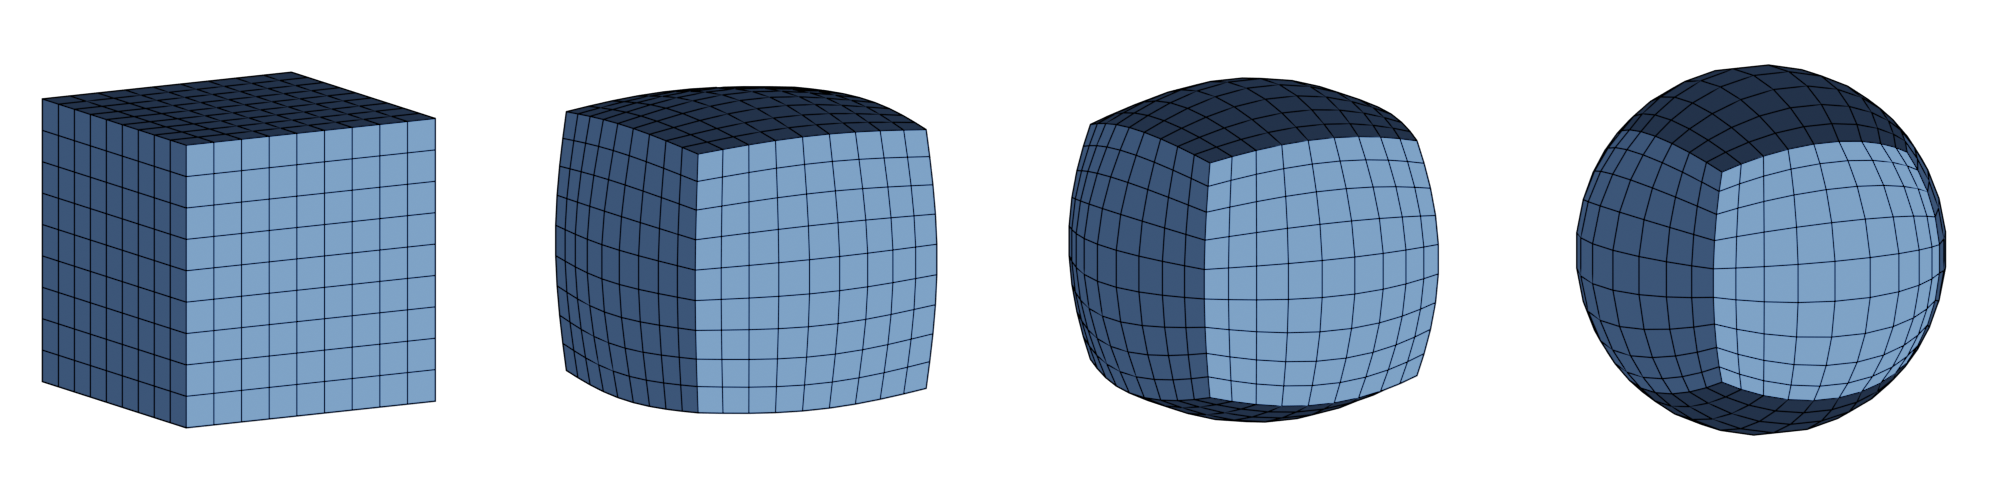
\includegraphics[width=0.7\linewidth]{Blender/CubeSphere.png}
        \caption{Deformation of a cube into a sphere.}
        \label{fig:cubesphere}
    \end{figure}
    \item Any knot can have a projection with as many crossings as desired.
    \item \textbf{Alternating knot}: \dq{A knot with a projection that has crossings that alternate between over and under as one travels around the knot in a fixed direction}{7}
    \begin{itemize}
        \item The trefoil is such a knot.
    \end{itemize}
    \item \emph{Exercise 1.7*}: By changing some of the crossings from over to under or vice versa, any projection of a knot can be made into a projection of the unknot$^[$\footnote{How can I \emph{show} something? How can I do these proofs? What kind of logic solves one of these?}$^]$. See Figure \ref{fig:knottotrivial}.
    \begin{figure}[h!]
        \centering
        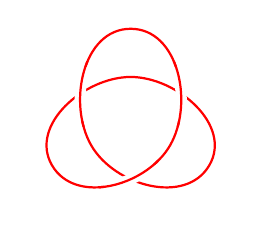
\begin{tikzpicture}
            \begin{knot}[
                consider self intersections,
                clip width=5
            ]
                \strand[red,thick] (1,{3^0.5})
                    to [out=0,in=60] (1.5,0.25)
                    to [out=240,in=-60] (0,0)
                    to [out=120,in=180] (1,1.12)
                    to [out=0,in=60] (2,0)
                    to [out=240,in=-60] (0.5,0.25)
                    to [out=120,in=180] cycle
                ;
                \flipcrossings{3}
            \end{knot}
        \end{tikzpicture}
        \caption{A projection of the unknot evoking the trefoil knot.}
        \label{fig:knottotrivial}
    \end{figure}
\end{itemize}


\subsection{Composition of Knots}
\begin{itemize}
    \item \dq{hi}{\#\#}
\end{itemize}




\end{document}



% \subsection{Reidemeister Moves}
% \begin{itemize}
%     \item \dq{hi}{\#\#}
% \end{itemize}


% \subsection{Links}
% \begin{itemize}
%     \item \dq{hi}{\#\#}
% \end{itemize}


% \subsection{Tricolorability}
% \begin{itemize}
%     \item \dq{hi}{\#\#}
% \end{itemize}


% \subsection{Knots and Sticks}
% \begin{itemize}
%     \item \dq{hi}{\#\#}
% \end{itemize}